\documentclass[10pt,letterpaper]{article}
\usepackage[dvipsnames]{xcolor}
\usepackage{outlines}
\usepackage{amsmath}
\usepackage{tikz}
\usepackage{hyperref}
\usepackage{enumitem}
\usepackage{cancel}
\usepackage{subcaption}
\DeclareCaptionOptionNoValue{centering}{\centering} % Make sure everything is centered in subs
\captionsetup[sub]{centering}

\usepackage{algorithm}
\usepackage[noend]{algpseudocode}
\makeatletter
\def\BState{\State\hskip-\ALG@thistlm}
\makeatother

\usepackage{multirow}
\usepackage{cancel}
\usepackage{float}

\usepackage{parskip}

\usepackage{slantsc,lmodern}

\usepackage{pgfplotstable,booktabs}
\usepackage{framed}
\definecolor{shadecolor}{rgb}{0.9,0.9,0.9}

\usepackage{gensymb}

\usepackage{paralist}

\usepackage[paper=a4paper,margin=1in]{geometry}

\usepackage{etoolbox}

\newcommand{\volume}{{\ooalign{\hfil$V$\hfil\cr\kern0.08em--\hfil\cr}}}

\makeatletter
\g@addto@macro\@floatboxreset\centering
\makeatother

\author{Thaddeus Hughes \\ hughes.thad@gmail.com \\ thaddeus-maximus.github.io}
\date{\today}
\title{Documentation and Validation of EveryCalc's Trajectory Tool}



\begin{document}
	\maketitle
	
	\begin{abstract}
		Hurling projectiles is something we humans really like doing. We've become exceedingly efficient at it. We make sport of it. We can guess at a trajectory pretty easily- but nailing it down, and tweaking it with an engineering mindset is harder. Lots of tools already exist to do this but I want to roll my own so I can add all the physics I want, along with the swept area of a projectile, and stacking the tolerance.
	\end{abstract}
	
\section{Basic Projectile Motion}
	Consider a ball of mass $m$, in a vacuum. It has only the force of gravity acting on it. That is to say,

	\begin{align}
		\Sigma F_x &= m \frac{d v_x}{d t} = 0 \\
		\Sigma F_y &= m \frac{d v_y}{d t} = - m g
	\end{align}

	To figure out the path, we'd also need to know the initial conidtions. Let's also say that the ball was launched at an angle $\theta$ from the horizontal at an initial velocity of $\bar{v}_0$, so that the x- and y- velocities would be
	\begin{align}
		v_x(0) &= \bar{v}_0 \ cos(\theta) \\
		v_y(0) &= \bar{v}_0 \ sin(\theta) .
	\end{align}

	We'll start from a height of $y_0$ and at $x=-x_0$ from our target.

	\begin{align}
		x(0) = -x_0 \\
		y(0) = -y_0 
	\end{align}

	This is enough to get us a very simple simulation for projectile motion:

	\begin{align}
		\frac{d v_x}{d t} &= 0 \\
		\frac{d v_y}{d t} &= - g \\
		\frac{d x}{d t} &= v_x \\
		\frac{d y}{d t} &= v_y \\
		v_x(0) &= \bar{v}_0 \ cos(\theta) \\
		v_y(0) &= \bar{v}_0 \ sin(\theta) \\
		x(0) &= -x_0 \\
		y(0) &= y_0 \\
		\text{terminate when } x &\geq 0
	\end{align}

\section{Swept Path with Parallel Curves}
	It's also worth knowing the swept zone that the target travels, since the object of firing a projectile may not be to hit a target per se, but to make it \textit{through} a target. This may seem like a trivial task at first blush; just add on the radius of the ball to the y-direction, but then one realizes the projetile may not be striking the target dead-on. Creating an offset path, or \href{https://en.wikipedia.org/wiki/Parallel_curve}{parallel curve} is necessary. The upper swept path ($x_u$, $y_u$) of a ball of radius $r$ can be determined as

	\begin{align}
		x_u = x + r (\hat{x} \cdot \hat{N}) \\
		y_u = y + r (\hat{y} \cdot \hat{N})
	\end{align}

	Where $\hat{x}$, $\hat{y}$, $\hat{N}$, $\hat{T}$ are unit vectors in the x-, y-, normal, and tangent directions.

	\begin{align}
		\text{let } \bar{v} &= \sqrt{v_x^2 + v_y^2} \\
		\hat{x} \cdot \hat{N} &= - v_x / \bar{v} \\
		\hat{x} \cdot \hat{T} &= + v_y / \bar{v} \\
		\hat{y} \cdot \hat{N} &= + v_x / \bar{v} \\
		\hat{y} \cdot \hat{T} &= + v_y / \bar{v}
	\end{align}

	The lower path would be found by reversing the direction of $r$, yielding
	
	\begin{align}
		x_l &= x - r (\hat{x} \cdot \hat{N}) \\
		y_l &= y - r (\hat{y} \cdot \hat{N}) .
	\end{align}

\section{Aerodynamic Effects}
	There are multiple aerodynamic forces that can act on a ball.

	\begin{align}
		F_{drag}   &= \frac{1}{2}   \ C_{drag} \ \rho \ A \ \bar{v}^2 \\
		F_{lift}   &= \frac{1}{2}   \ C_{lift} \ \rho \ A \ \bar{v}^2 \\
		F_{magnus} &= \frac{\pi}{3} \ C_{magnus} \ \rho \ A \ \bar{v} \ \omega_{\text{+ccw}}
	\end{align}	

	The lift and drag forces are standard equations, but the magnus force equation is derived from \href{https://www.grc.nasa.gov/WWW/K-12/airplane/beach.html}{\underline{this NASA page}}. There are undoubtedly better models out there, but this is what I have currently.

	In vector form the conservation of momentum could be written as

	\begin{align}
		m \frac{d \vec{v}}{d t} = - F_{drag} \hat{T} + F_{lift} \hat{N} + F_{magnus} \hat{N} - m g \hat{y}
	\end{align}

	This changes the model, when projected out into the x- and y- components to

	\begin{align}
		\frac{d v_x}{d t} &= \frac{- F_{drag} (\hat{x} \cdot \hat{T}) + F_{lift} (\hat{x} \cdot \hat{N}) + F_{magnus} (\hat{x} \cdot \hat{N})}{m}\\
		\frac{d v_y}{d t} &= \frac{ - F_{drag} (\hat{y} \cdot \hat{T}) + F_{lift} (\hat{y} \cdot \hat{N}) + F_{magnus} (\hat{y} \cdot \hat{N})}{m} - g \\
		\frac{d x}{d t} &= v_x \\
		\frac{d y}{d t} &= v_y \\
		v_x(0) &= \bar{v}_0 \ cos(\theta) \\
		v_y(0) &= \bar{v}_0 \ sin(\theta) \\
		x(0) &= -x_0 \\
		y(0) &= y_0 \\
		\text{terminate when } x &\geq 0 .
	\end{align}

\section{Tolerance Stacking}
	To determine accuracy, multiple iterations of the simulation can be ran with different permutations of input variables.

\section{Reverse Computation}
	A \href{https://en.wikipedia.org/wiki/Bisection_method}{\underline{bisection algorithm}} is used to solve for the appropriate distance/angle/velocity required to propel the projectile into the target. This has benefits over analytical solutions in that it can be used in conjunction with aerodynamic effects.

\section{Validation Against Other Tools}

	I'll compare results to \href{https://www.chiefdelphi.com/t/amb-design-spreadsheet-v5/383857}{\underline{AMB's Design Spreadsheet}}.

	\newpage
	\subsection*{Case A: Metric units, no aero}

	\begin{figure}[H]
		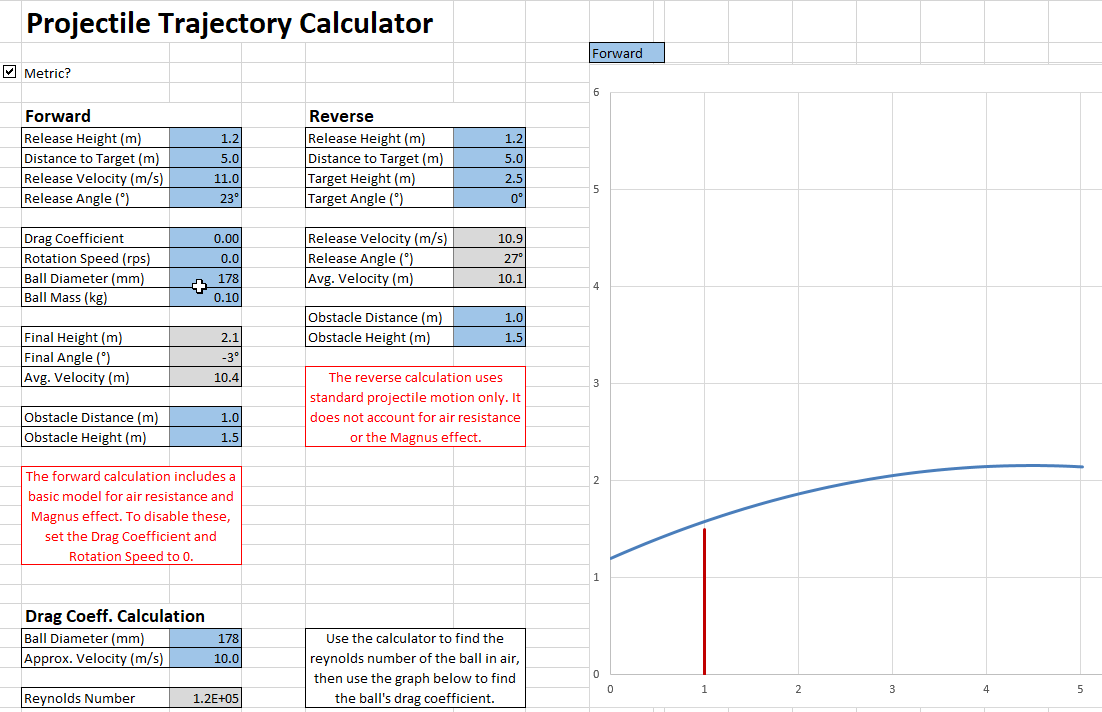
\includegraphics[width=0.8\textwidth]{validation/trajectory_AMB_A.png}
	\end{figure}

	\begin{figure}[H]
		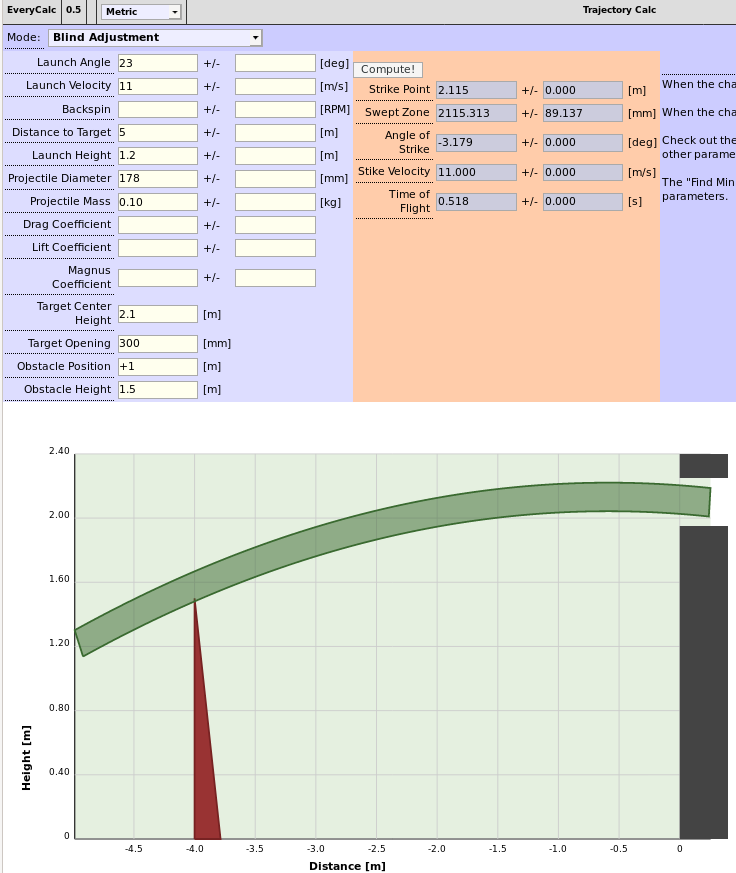
\includegraphics[width=0.65\textwidth]{validation/trajectory_EC_A.png}
	\end{figure}

	Look only at the "Forward" portions of AMB's sheet. Effectively the same result.

	\newpage
	\subsection*{Case B: English units, drag included}
	\begin{figure}[H]
		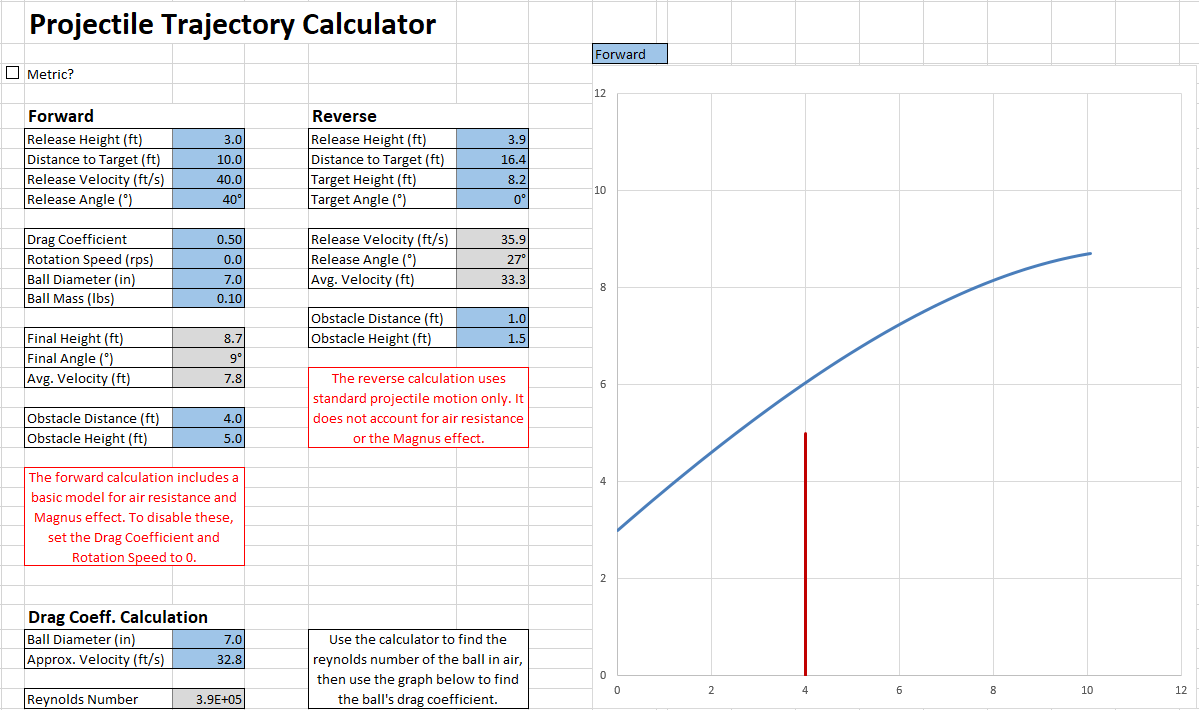
\includegraphics[width=0.8\textwidth]{validation/trajectory_AMB_B.png}
	\end{figure}

	\begin{figure}[H]
		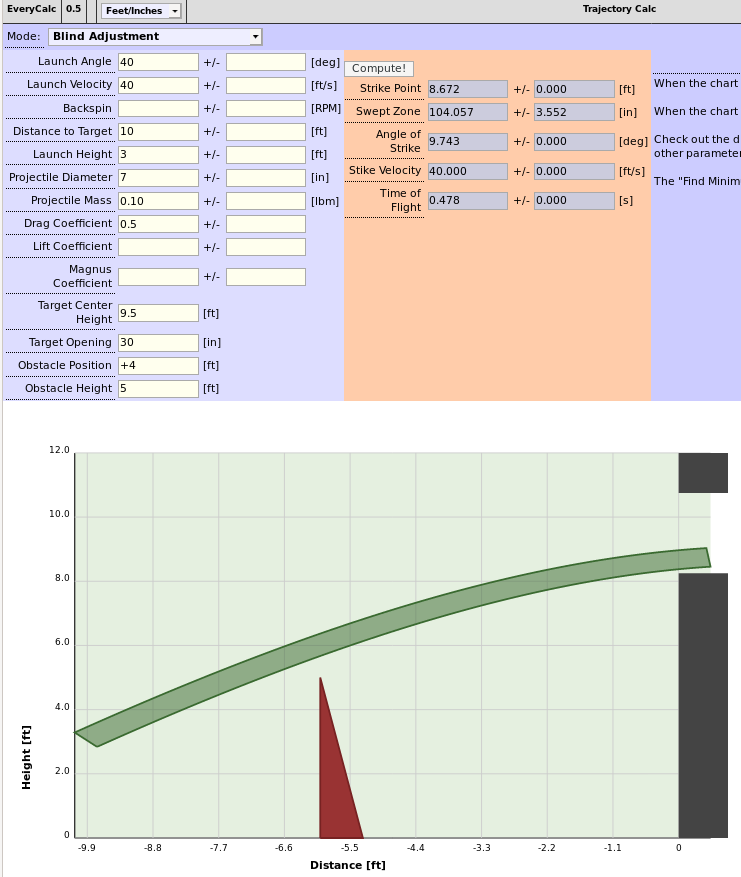
\includegraphics[width=0.65\textwidth]{validation/trajectory_EC_B.png}
	\end{figure}

	Look only at the "Forward" portions of AMB's sheet. Effectively the same result.
	
\end{document}